% !TEX program = xelatex
% 复现自 CV——AI infra.pdf（BabelDOC/PyMuPDF span 级解析：字体、字号、颜色、坐标）
% 字体优先级：SimSun/KaiTi/Times New Roman（与原版一致）→ 无原字体机器自动回退
\documentclass[a4paper]{article}

\usepackage[a4paper,left=30pt,right=17pt,top=22.5pt,bottom=15pt,nohead,nofoot]{geometry}
\usepackage{fontspec}
\usepackage{xeCJK}
\usepackage{xcolor}
\usepackage{tikz}
\usetikzlibrary{calc}

% ---------- 字体 ----------
\setmainfont{Times New Roman} % 原版拉丁字体
% CJK 字体探测：Windows 有 SimSun/KaiTi 原字体；其它环境回退到开源近似字体
\IfFileExists{C:/Windows/Fonts/simkai.ttf}{%
  \setCJKmainfont{KaiTi}[AutoFakeBold=3]%
  \newCJKfontfamily\songti{SimSun}[AutoFakeBold=3]%
}{%
  \setCJKmainfont{AR PL UKai CN}[AutoFakeBold=3]%
  \newCJKfontfamily\songti{Noto Serif CJK SC}[AutoFakeBold=3]%
}

% ---------- 颜色（逐 span 采样值） ----------
\definecolor{headpurple}{HTML}{660773} % 节标题文字
\definecolor{rulepurple}{HTML}{6F2F9F} % 节标题分隔线
\definecolor{bodygray}{HTML}{404040}   % 正文/日期

% ---------- 版式常量 ----------
\newcommand{\bodyfont}{\fontsize{9.96}{12}\selectfont\color{bodygray}} % 正文：9.96pt/12pt
\newcommand{\cvsection}[2][0pt]{%
  \par\vspace{3.2pt}\noindent
  \hspace{#1}{\songti\bfseries\fontsize{11.04}{12}\selectfont\color{headpurple}#2}%
  \par\nointerlineskip\vspace{0.5pt}%
  \noindent\hspace{5pt}\smash{\textcolor{rulepurple}{\rule{525pt}{1.05pt}}}%
  \par\nointerlineskip\vspace{2.5pt}}

\newcommand{\datemonth}[2]{\textbf{#1}{年}\textbf{#2}{月}} % 数字 Times 粗体，年月楷体常规
\newcommand{\daterange}[2]{\datemonth{#1}{#2}}
\newcommand{\para}{\par\noindent\hspace{13.3pt}}           % 条目缩进（符号图标位）
\newcommand{\compitem}{\par\noindent\hspace{20.2pt}}       % 竞赛条目缩进
\newcommand{\rightdate}[1]{\hfill\makebox[0pt][r]{\bodyfont #1}\hspace{13pt}}

\pagestyle{empty}
\setlength{\parindent}{0pt}
\setlength{\parskip}{0pt}
\linespread{1}

\begin{document}
% ---------- 页眉装饰图（原版绝对位置） ----------
\begin{tikzpicture}[remember picture,overlay]
  \node[anchor=north west,inner sep=0] at
    ([xshift=26pt,yshift=-31.8pt]current page.north west)
    {
\includegraphics[width=129.2pt]{header_left.jpg}};
  \node[anchor=north west,inner sep=0] at
    ([xshift=492pt,yshift=-5.5pt]current page.north west)
    {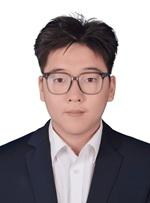
\includegraphics[width=69.5pt]{header_right.jpg}};
\end{tikzpicture}%

% ---------- 姓名区 ----------
{\centering
{\songti\bfseries\fontsize{15}{15}\selectfont\color{black}姚润泽}\\[4.9pt]
{\bodyfont 政治面貌：中共党员}\\[6.9pt]
{\bodyfont 联系方式 +86-177-5315-8846 丨 邮箱：y17753158846@outlook.com}\par}

% ---------- 教育经历 ----------
\cvsection{教育经历}
\bodyfont
\para 本科：东北大学（\textbf{985}）\hspace{3pt} 自动化（\textbf{A+}） （2022-2026）

\para 博士研究生：清华大学\hspace{2pt} 电子信息\hspace{2pt} （2026-2031）

\para 研究方向：AI Infra

\para 英语能力：六级 514 分，四级 586 分

\para 技术栈：P4、模型压缩、分布式训练系统、实时推理优化

% ---------- 科研经历 ----------
\cvsection{科研经历}

\noindent\hspace{5pt}{\fontsize{10.56}{12.3}\selectfont\color{black}%
Facilitating Low-Resource Complex In-network Traffic Classification and Incremental Update via LLM-inspired Hierarchical Trainining}%
\rightdate{\datemonth{2025}{02}\ -\ \datemonth{2025}{11}}
\vspace{2.1pt}

\bodyfont
\para 项目目标：针对大语言模型（LLM）在网络边缘侧设备面临的计算资源匮乏、异质硬件部署困难等核心痛点，研究并设计了一套基于 LLM 驱动的自动化任务编排与轻量化层次推理架构，旨在打通云端高层语义智能与底层数据面线速性能之间的技术壁垒。

\para 创新点：(1)基于智能体的任务自动化编排：创新性地引入 LLM 专家智能体，利用思维链（Chain-of-Thought, CoT）机制将复杂的网络分类逻辑自动解耦为层次化的子任务。构建了基于多智能体（Multi-Agent）协同的 Actor-Critic 模式，通过对分解策略进行动态评估与闭环优选，彻底替代了传统依赖专家经验的人工特征工程。(2)多分支神经网络单元（NNU）设计：针对数据面硬件特性设计了多分支 NNU 结构，将 LLM 的通用推理能力有效蒸馏为可直接下发的轻量化匹配规则。该架构不仅支持面向新流量模式的 Few-Shot（小样本）增量更新，更确保了模型在可编程硬件上能够维持线速（Line-rate）推理，实现了高精度与高吞吐的平衡。

\para 成果产出：成功实现了从大模型逻辑规划到边缘侧（\textbf{P4 Switch}）落地执行的全流程闭环系统原型。相关实验数据验证了架构的灵活性与资源高效性，研究成果已投稿至 CCF-A 类国际顶刊 IEEE Transactions on Networking (一作返修中)。

\vspace{4.2pt}
\noindent\hspace{5pt}{\songti\fontsize{9}{11}\selectfont\color{black}面向异构数据面的弹性流量分析与自动化部署机制研究}%
\rightdate{\datemonth{2025}{08}\ -\ \datemonth{2026}{01}}

\bodyfont
\para 项目目标：针对流量分析模型在异构数据面（Tofino/eBPF/BMV2）部署时面临的资源异质性与重训练高昂成本，设计基于“模型-硬件解耦”思想的自动化编译与弹性适配架构。

\para 创新点：1）弹性推理架构 (Elastic Inference)：提出 Elastic Decision Tree (EDT) 范式，融合知识蒸馏与软硬协同剪枝算法，在零重训练（Zero-Retraining）前提下实现模型结构对流水线级数与存储资源的动态适配；2）约束驱动的自动编排：构建基于回归树的细粒度资源预测模型（RMSE < 1.7\%），提出单调资源搜索遗传算法 (Hierarchical GA)，在满足 TCAM/SRAM/Stage 多维硬约束下自动搜索特征匹配与拓扑结构的最优帕累托解。

\para 成果：依托国家自然科学基金项目，开发了跨平台自动化编排原型系统。经 Tofino/bmv2 真实环境验证，在极端资源受限场景下，相比 SOTA 方案部署成功率提升 100\%。相关理论与实验成果拟投稿至 CCF-A 类期刊《IEEE ToN》。

\vspace{4.2pt}
\noindent\hspace{5pt}{\songti\fontsize{9}{11}\selectfont\color{black}面向大规模分布式训练的弹性聚合与高效通信机制研究}%
\rightdate{\datemonth{2026}{02}\ -\ 至今}

\bodyfont
\para 项目目标：针对大规模分布式训练中参数同步的通信瓶颈与单点故障问题，设计基于跨节点资源借用的弹性聚合架构，将碎片化空闲资源组织为瞬时缓冲池，为局部通信失败提供低开销容错路径，支撑大规模 Model 的可靠分布式训练。

\para 创新点：(1) 双角色路径锁定与单跳转发协议：设计 source/guest 双角色路径锁定机制，首包裁决后同 tuple 严格复用路径，以 sealed 状态机实现 per-tuple 粒度的槽位回收，保障大规模参数同步的低延迟与高可靠。(2) 定向恢复与轻量协议设计：将故障恢复局部化至任务粒度，仅向受影响节点定向拉取部分数据，避免全局重传；设计轻量协议头集成状态管理字段，在有限带宽内实现高效同步控制。

\para 成果：此研究为内网聚合的弹性容错提供了新的设计范式，在设计上区别于现有分布式训练通信系统的集中式回退路径。

% ---------- 竞赛经历 ----------
\cvsection[5.2pt]{竞赛经历}

\noindent\hspace{5.1pt}{\songti\fontsize{10.56}{12}\selectfont\color{bodygray}国家奖项五项，省级奖项十余项，采取部分奖项展示：}

\bodyfont
\compitem 第十九届全国大学生智能汽车竞赛全国总冠军（室外赛无人驾驶自行车组）\rightdate{\textbf{2024} 年\textbf{09} 月 - \textbf{2024} 年\textbf{12} 月}

\compitem 第十九届全国大学生智能汽车竞赛国家一等奖（基础赛独轮组）\rightdate{\textbf{2023} 年\textbf{12} 月 - \textbf{2024} 年\textbf{08} 月}

\compitem 第十九届全国大学生智能汽车竞赛国家二等奖（创意赛天途智慧救援组）\rightdate{\textbf{2024} 年\textbf{04} 月 - \textbf{2024} 年\textbf{08} 月}

\compitem 第十二届中国 triz 杯大学生创新方法大赛国家三等奖（生活创意赛道）\rightdate{\textbf{2024} 年\textbf{03} 月 - \textbf{2024} 年\textbf{07} 月}

\compitem 第十八届“西门子杯”中国智能制造挑战赛省级二等奖（流程行业自动化组）\rightdate{\textbf{2023} 年\textbf{12} 月 - \textbf{2024} 年\textbf{08} 月}

\compitem 第十五届蓝桥杯全国软件和信息技术专业人才大赛省级二等奖（单片机组）\rightdate{\textbf{2023} 年\textbf{12} 月 - \textbf{2024} 年\textbf{05} 月}

% ---------- 个人优势 ----------
\cvsection[5.2pt]{个人优势}
\bodyfont
\para AI 系统全栈：在 IEEE ToN 工作中主导神经网络→可编程硬件的自动编译方案设计（知识蒸馏、特征选择、增量学习）；\\[4.1pt]
\hspace*{13.3pt}在异构场景需求下实现遗传算法驱动的多目标编译优化，打通算法→编译器→硬件完整链路。

\vspace{0.7pt}
\para 系统性能优化：熟练 Python/P4，对 PyTorch、分布式通信（聚合/AllReduce）及可编程边缘设备有实战经验；独立设计跨节点弹性聚合协议，方法论可迁移至大规模分布式训练场景。

\para 工程落地与跨领域迁移：具备在学术研究与系统工程之间形成闭环的工作习惯，在 CCF-A 类期刊上产出论文的同时，持续将算法方案落地至真实硬件完成端到端验证，确保理论成果经得起实践检验。这种研究方式使编译器设计、分布式优化等底层系统方法论能够自然迁移至 GPU 算子开发、大模型推理加速等新方向，辅以丰富的硬核竞赛经历对全栈交付能力的长期锤炼，可在 AI Infra 及相关领域快速上手掌握。

% ---------- 其他 ----------
\cvsection[5.2pt]{其他}
\bodyfont
\begin{minipage}[t]{0.591\textwidth}
2026 年东北大学优秀毕业生
\end{minipage}%
\begin{minipage}[t]{0.591\textwidth}
\hspace{0pt}2026 年东北大学就业之星（升学类）
\end{minipage}

\vspace{0.7pt}
\begin{minipage}[t]{0.591\textwidth}
2024 年11 月优秀学生干部
\end{minipage}%
\begin{minipage}[t]{0.591\textwidth}
2024 年5 月优秀团干部标兵
\end{minipage}

\begin{minipage}[t]{0.591\textwidth}
2024 年3 月创新创业工作优秀学生干部
\end{minipage}%
\begin{minipage}[t]{0.591\textwidth}
2023 年11 月三好学生
\end{minipage}

\begin{minipage}[t]{0.591\textwidth}
2023 年11 月志愿服务之星
\end{minipage}%
\begin{minipage}[t]{0.591\textwidth}
2023 年5 月优秀团员
\end{minipage}

\end{document}
